%
\section{Testen}

\subsection{Testen der Methode \textit{IsWithinConstructorOf}}
In C\# 6 können Auto-Properties ohne Setter deklariert werden.\cite{csharp6} C\# Essentials überprüft, ob der Setter weggelassen werden kann und teilt dies gegebenenfalls dem Benutzer mit. Die zu testende Methode \textit{IsWithinConstructorOf} überprüft dabei, ob das Setzen des Auto-Properties im Konstruktor stattfindet. Die statische Analyse ergab, dass diese Methode sehr Komplex und damit sehr fehleranfällig ist. Daher haben wir uns entschlossen diese genauer zu testen. Dazu haben wir, den in Abbildung~\ref{fig:graph-constructor} dargestellten, Kontrollflussgraphen erstellt. Anschließend haben wir folgende Testpfade für unterschiedliche Coverage Kriterien entwickelt.\\
\begin{figure}
	\centering
	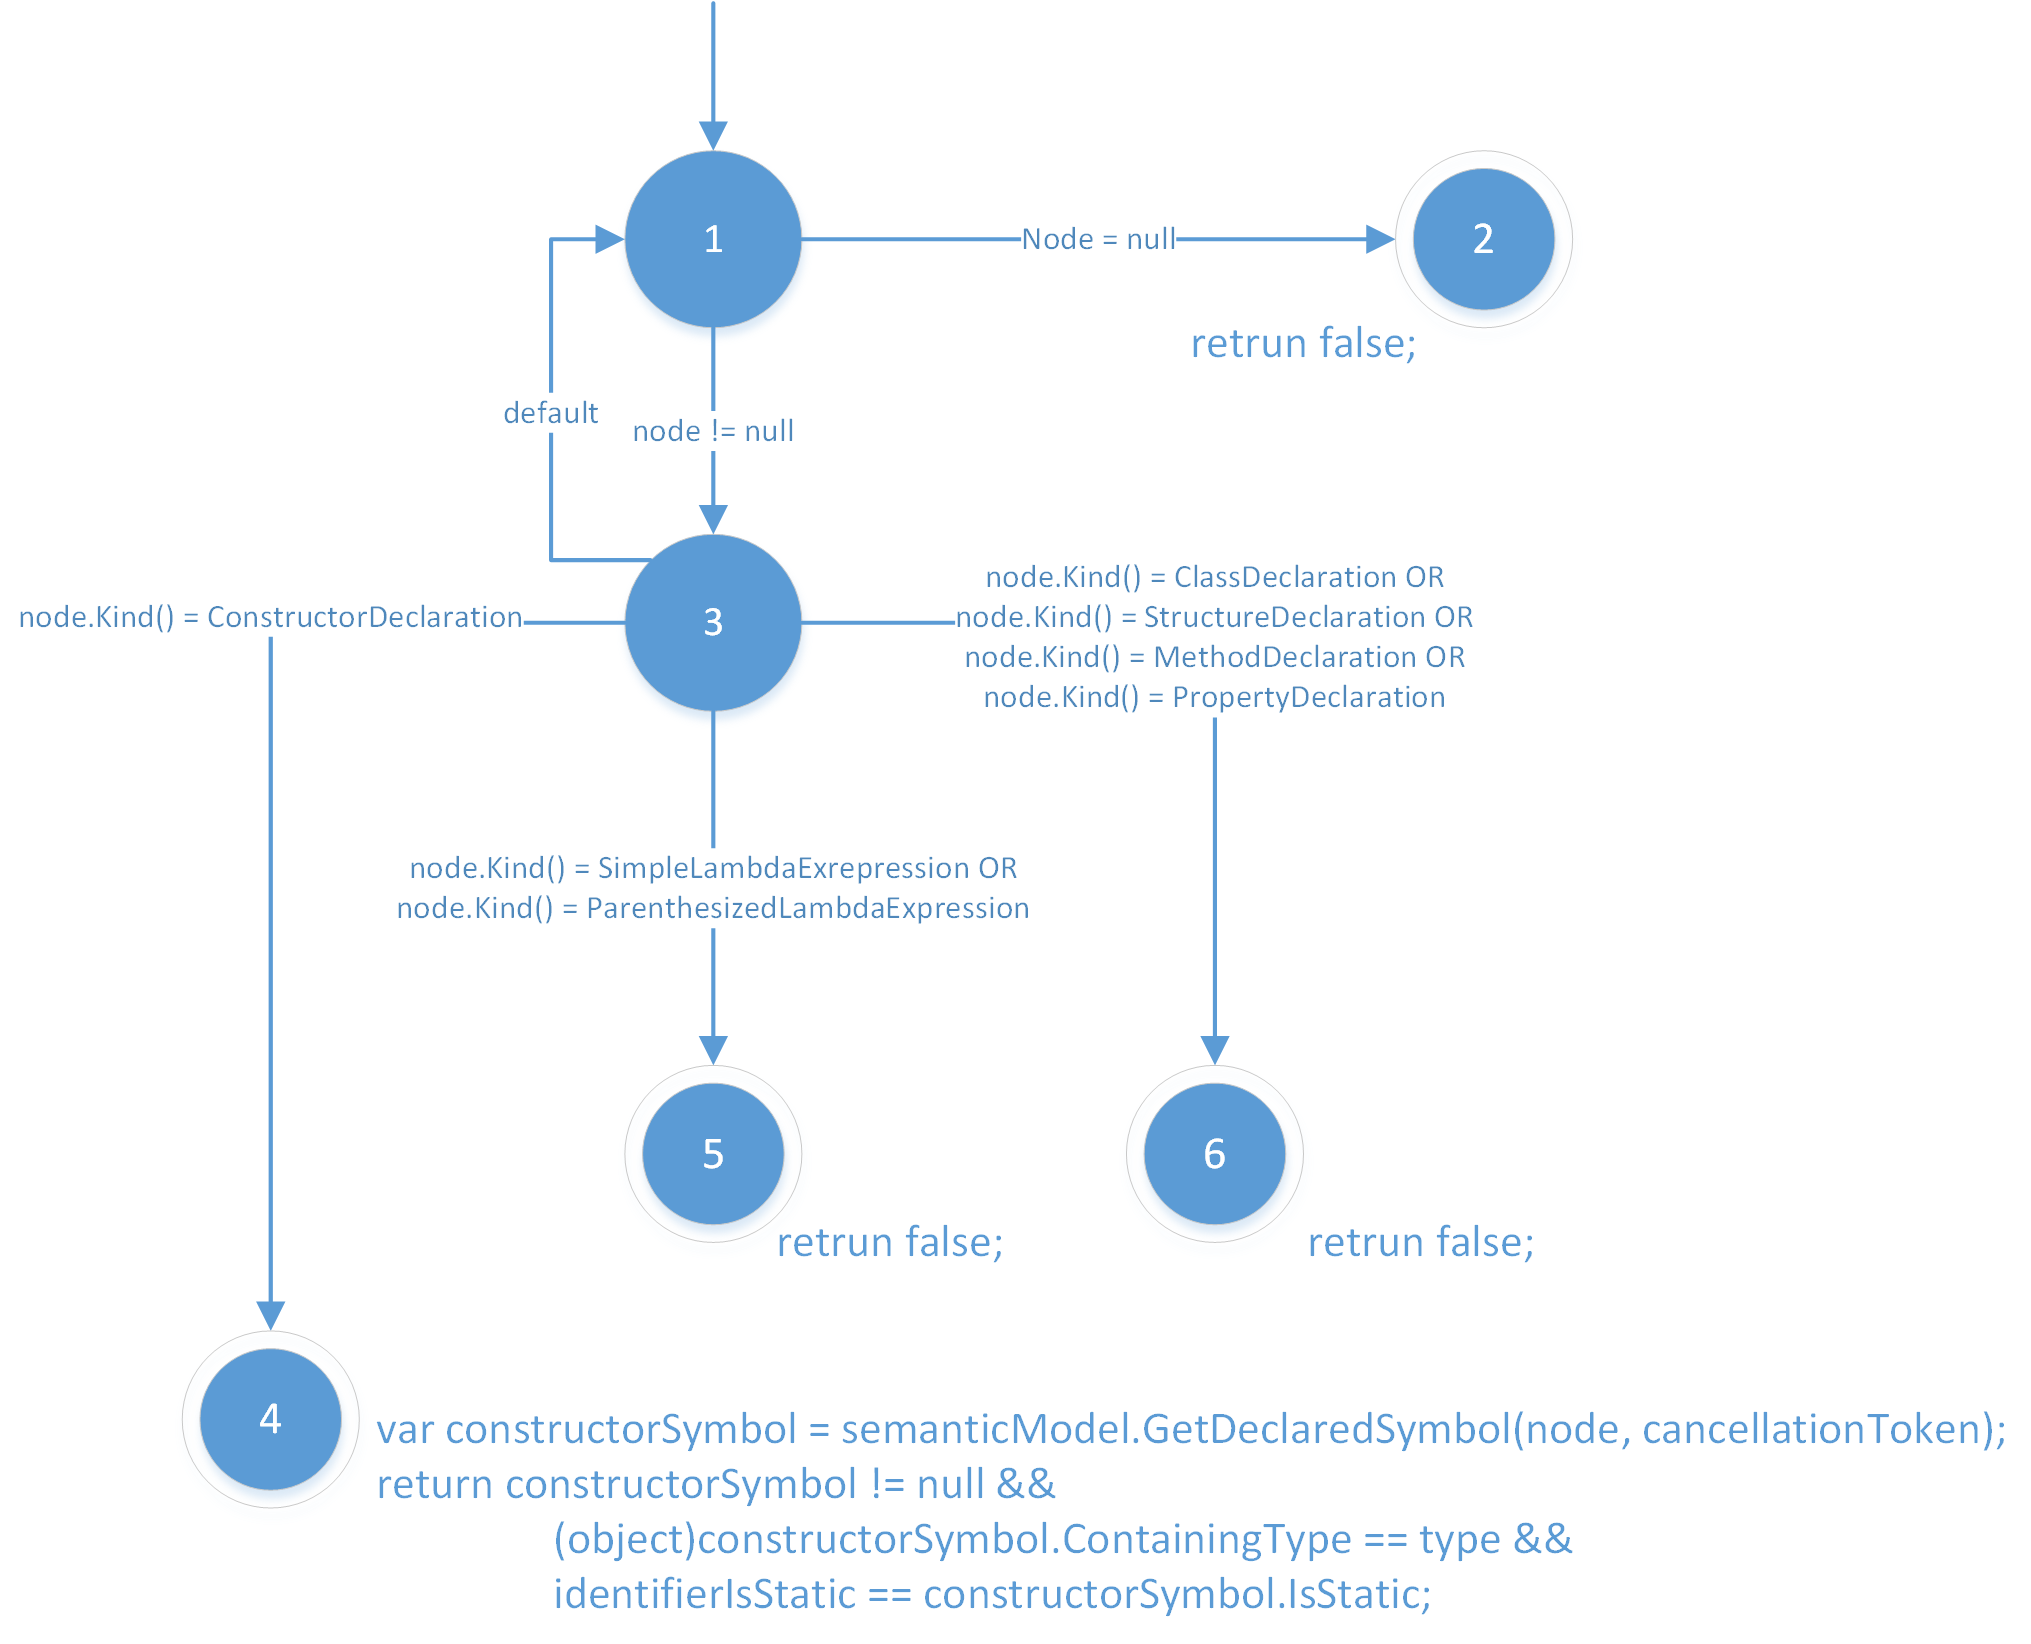
\includegraphics[width=\textwidth]{images/GraphIsWithinConstructorOf.png}
	\caption{Graph für die Methode \textit{IsWithinConstructorOf}()}
	\label{fig:graph-constructor}
\end{figure}
\lstset{caption={Coverage für die Mehtode \textit{IsWithinConstructorOf}}}
\begin{lstlisting}
Node Coverage:
TR = {1,2,3,4,5,6}
Example Test Paths = [1,3,4], [1,3,5], [1,3,6]

Edge Coverage:
TR = {(1,2), (1,3), (3,1), (3,4), (3,5), (3,6)}
Example Test Paths = [1,3,1,2], [1,3,4], [1,3,5], [1,3,6]

Edge Pair Coverage:
TR = {[1,3,1], [1,3,4], [1,3,5], [1,3,6], [3,1,3], [3,1,2]}
Example Test Paths = [1,3,1,3,1,2], [1,3,4], [1,3,5], [1,3,6]

Prime Path Coverage:
TR = {[1,3,4], [1,3,5], [1,3,6], [3,1,2], [3,1,3], [1,3,1]}
Example Test Paths: [1,3,1,3,1,2], [1,3,4], [1,3,4], [1,3,5]

\end{lstlisting}
\vspace{3ex}
Zu erkennen ist, dass Edge Pair und Prime Path Coverage die selben Test Paths besitzen. Abschließend haben wir für die Methode \textit{IsWithinConstructorOf} jeweils einen Test programmiert, der einen der Testpfade der Prime beziehungsweise Edge Pair Coverage abdeckt.


\subsection{Testen der Methode \textit{IsValidStringFormatMethod}}
C\# 6 unterstützt interpolated Strings. Anstatt in der \textit{String.Format} Methode Platzhalter zu verwenden, um Variablen einzufügen, können diese nun direkt im String verwendet werden.\cite{csharp6} C\# Essentials gibt dem Benutzer Vorschläge, wie er die neuen interpolated Strings verwendet. Die Methode \textit{String.Format} überprüft in diesem Zusammenhang, wann es sich um ein valide \textit{String.Format} Methode handelt.\\
Auch beim Testen dieser Methode haben wir zu erst den Kontrollflussgraphen, wie in Abbildung \ref{fig:graph-validstring} zu sehen, erzeugt. Anschließend haben wir die folgenden Coverage Kriterien aufgestellt.
\lstset{caption={Coverage für die Mehtode \textit{IsValidStringFormatMethod}}}
\begin{lstlisting}
Node Coverage:
TR = {1,2,3,4,5,6,7}
Example Test Paths = [1,2], [1,3,4], [1,3,5,6], [1,3,5,7]

Edge Coverage:
TR = {(1,2), (1,3), (3,4), (3,5), (5,6), (5,7)}
Example Test Paths = [1,2], [1,3,4], [1,3,5,6], [1,3,5,7]

Edge Pair Coverage:
TR = {[1,2], [1,3,4], [1,3,5], [3,5,6], [3,5,7]}
Example Test Paths = [1,2], [1,3,4], [1,3,5,6], [1,3,5,7]

Prime Path Coverage:
TR = {[1,2], [1,3,4], [1,3,5,6], [1,3,5,7]}
Example Test Paths: [1,2], [1,3,4], [1,3,5,6], [1,3,5,7]

\end{lstlisting}

\begin{figure}
	\centering
	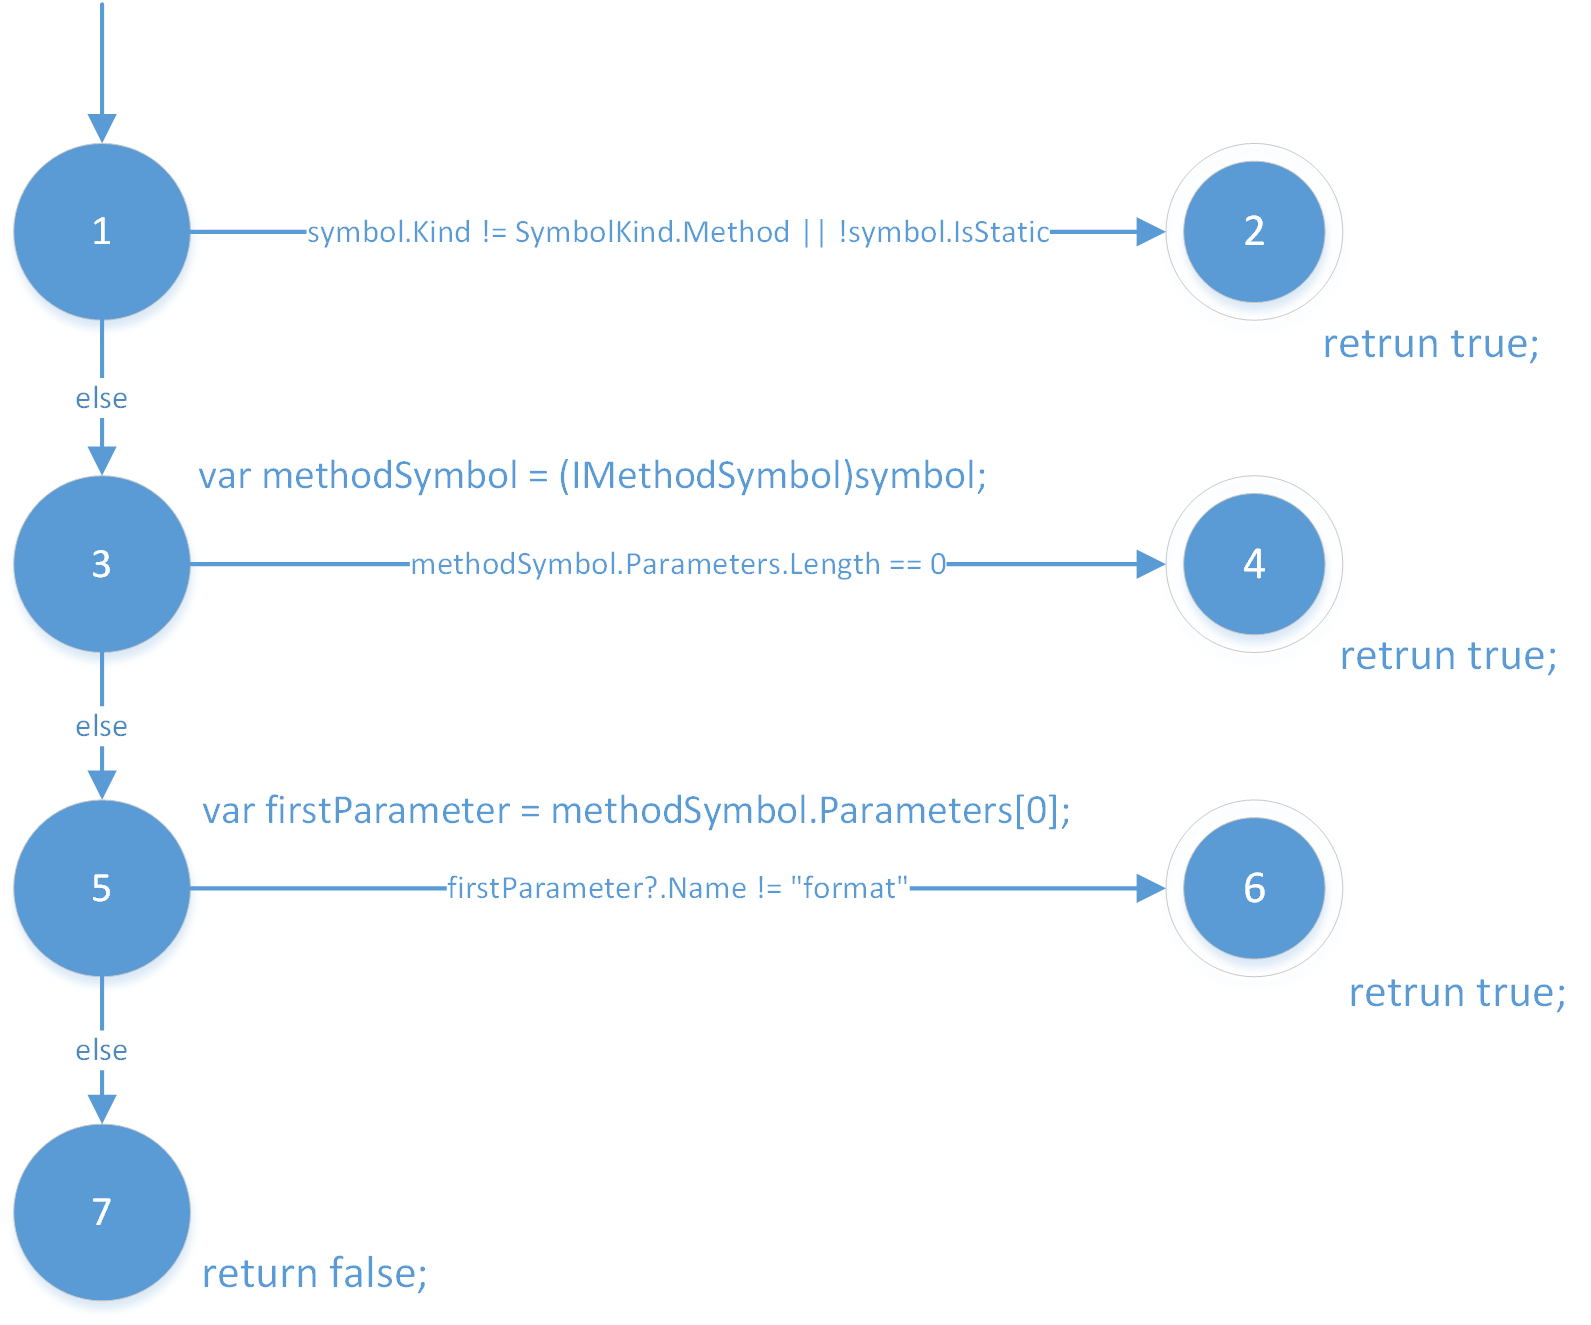
\includegraphics[width=0.8\textwidth]{images/GraphISValidStringFormatMethod.png}
	\caption{Graph für die Methode \textit{IsValidStringFormatMethod}()}
	\label{fig:graph-validstring}
\end{figure}
\definecolor{bluekeywords}{rgb}{0.13,0.13,1}
\definecolor{greencomments}{rgb}{0,0.5,0}
\definecolor{redstrings}{rgb}{0.9,0,0}
\definecolor{light-gray}{gray}{0.96}
\lstset{language=[Sharp]C,
	showspaces=false,
	showtabs=false,
	breaklines=true,
	showstringspaces=false,
	breakatwhitespace=true,
	escapeinside={(*@}{@*)},
	commentstyle=\color{greencomments},
	keywordstyle=\color{bluekeywords},
	stringstyle=\color{redstrings},
	basicstyle=\ttfamily,
	tabsize=2,
	 backgroundcolor=\color{light-gray},
	caption={Mehtode \textit{IsWithinConstructorOf}}
}
\begin{lstlisting}
private static bool IsWithinConstructorOf(SyntaxNode node, INamedTypeSymbol type, bool identifierIsStatic, SemanticModel semanticModel, CancellationToken cancellationToken)
{
	// Are we in a constructor?
	for (; node != null; node = node.Parent)
	{
		switch (node.Kind())
		{
			case SyntaxKind.ConstructorDeclaration:
				// In a constructor. Is it the constructor for the type that contains the property?
				var constructorSymbol = semanticModel.GetDeclaredSymbol(node, cancellationToken);
				return constructorSymbol != null && (object)constructorSymbol.ContainingType == type && identifierIsStatic == constructorSymbol.IsStatic;
			// If it's in a lambda expression, even if in a constructor, then it counts as a non-constructor case.
			case SyntaxKind.SimpleLambdaExpression:
			case SyntaxKind.ParenthesizedLambdaExpression:
				return false;
			// Early out cases. There are many others, but these are the common ones.
			case SyntaxKind.ClassDeclaration:
			case SyntaxKind.StructDeclaration:
			case SyntaxKind.MethodDeclaration:
			case SyntaxKind.PropertyDeclaration:
				return false;
		}
	}
	return false;
}
\end{lstlisting}
\lstset{language=[Sharp]C,
	showspaces=false,
	showtabs=false,
	breaklines=true,
	showstringspaces=false,
	breakatwhitespace=true,
	escapeinside={(*@}{@*)},
	commentstyle=\color{greencomments},
	keywordstyle=\color{bluekeywords},
	stringstyle=\color{redstrings},
	basicstyle=\ttfamily,
	tabsize=2,
	backgroundcolor=\color{light-gray},
	caption={Mehtode \textit{IsValidStringFormatMethod}}
}
\begin{lstlisting}

private static bool IsValidStringFormatMethod(ISymbol symbol)
{
	if (symbol.Kind != SymbolKind.Method || !symbol.IsStatic)
	{
		return true;
	}
	var methodSymbol = (IMethodSymbol)symbol;
	if (methodSymbol.Parameters.Length == 0)
	{
		return true;
	}
	var firstParameter = methodSymbol.Parameters[0];
	if (firstParameter?.Name != "format")
	{
		return true;
	}
	return false;
}
\end{lstlisting}
